
\documentclass[12pt]{amsart}

%%useful packages.  All fonts/symbols until color package.
\usepackage{latexsym}
\usepackage{amsthm}
\usepackage{enumitem}
\usepackage{amssymb}
\usepackage{amsmath}
\usepackage{amsfonts}
\usepackage{mathrsfs}
\usepackage{color}        %lots of colors
\usepackage{tikz}          %For drawing stuff
\usetikzlibrary{positioning,shapes,shadows}
\usetikzlibrary{arrows,automata}
\usepackage{float}         %Helps with positioning of figures
\usepackage{verbatim}   %allows commenting out large parts of text.  See the TODO list below.
\usepackage{caption}
\usepackage{subcaption}
\usepackage{xcolor}
\newcommand{\cpb}[1]{\textcolor{purple}{cpb: #1}}


%% setup for theorem environments
\def\newtheorems{\newtheorem{theorem}[subsection]{Theorem}
                \theoremstyle{definition}
                \newtheorem{algorithm}[subsection]{Algorithm}
                \newtheorem{cor}[subsection]{Corollary}
                \newtheorem{prop}[subsection]{Proposition}
                \newtheorem{lemma}[subsection]{Lemma}
                \newtheorem{definition}[subsection]{Definition}
                \newtheorem{notation}[subsection]{Notation}
                \newtheorem{convention}[subsection]{Convention}
                \newtheorem{claim}[subsection]{Claim}
                \newtheorem{sublemma}[subsection]{Sublemma}
                \theoremstyle{definition}
                \newtheorem{example}[subsection]{Example}
                \newtheorem{examples}[subsection]{Examples}
                \theoremstyle{definition}
                \newtheorem{remark}[subsection]{Remark}
                %\newtheorem{question}[theorem]{Question}
                \newtheorem{question}[section]{Question}
                \newtheorem{conjecture}[section]{Conjecture}}
\newtheorems

\newcommand{\seteq}{:=}
\newcommand{\wh}[1]{\widehat{#1}}
\newcommand{\CS}{\mathfrak{C}}
\newcommand{\CCn}{\mathfrak{C}_n}    %My Cantor space symbol
\newcommand{\CCk}[1]{\mathfrak{C}_{#1}}  %with a variable

% New commands involving mathoperators (which usually are in upright font in math mode)
\newcommand{\aut}{\mathop{\mathrm{Aut}}\nolimits}
\newcommand{\out}{\mathop{\mathrm{Out}}\nolimits}
\newcommand{\homeo}{\mathop{\mathrm{Homeo}}\nolimits}


\newcommand{\N}{\mathbb{N}}
\newcommand{\Z}{\mathbb{Z}}

% Tree stuff
\newcommand{\T}{\mathcal{T}}
\newcommand{\tn}{\T_n}
\newcommand{\D}{\mathcal{D}}
\newcommand{\R}{\mathcal{R}}
\newcommand{\s}{\mathcal{S}}
\newcommand{\xn}{X_n}
\newcommand{\xns}{X_n^*}
\newcommand{\Cn}{\mathfrak{C}_n}
\newcommand{\Ctwo}{\mathfrak{C}_2}
\newcommand{\xnomega}{X_n^{\omega}}

% Operators
\DeclareMathOperator{\chain}{chain}
\DeclareMathOperator{\suff}{suff}

% the title in square brackets is like a short title for pages in the middle of paper in a journal
% title in braces is the formal title.
\title[]{An algorithm to obtain Revealing Pairs of elements of Thompson's Group $V$}
\author{}

\begin{document}

\maketitle
\vspace{.2 in}


\tableofcontents

\section{Introduction}

    \section{Alphabets, Words, and Prefixes}
        
                Let $n\in \Z_{>1}$ be given, and let $X_n$ be the set $X_n:=\{0,1,\ldots, n-1\}$.  We will refer to $X_n$ as \textit{the ($n$-ary) alphabet}.

   Let $\xns$ denote the set of all finite strings of elements in $\xn$, including the empty string $\varepsilon$, called \textit{words}. We also use $\xnomega$ to represent the set of infinite strings over $\xn$ (each such string can be thought of as a function from the limit ordinal $\omega$ to $\xn$).
        
        For any words $ w  \in \xns$ and $ v  \in X^\omega \cup \xns$, write $ w   v $ as the \textit{concatenation} of two strings (the string created by starting with the string $w$ and then continuing with the string $v$). We say that $ w  \in \xns$ is a \textit{prefix} of $ v  \in X^\omega  \cup \xns$ if there exists some $y \in X^ w  \cup \xns$ such that $ v  =  w y$, denoted $ w  \preceq  v $ (or $ w  \prec  v $ if it is known that $y \neq \varepsilon$).  We refer to $\preceq$ as the \textit{prefix relation (on $\xns$)}.  We will also denote by $\mid w \mid$ the length of any given word $ w $ (e.g. $\mid\varepsilon\mid=0$ and $\mid0110\mid=4$).
        
         If we give $\xn$ the discrete topology, then $X^\omega $ is an infinite product space and this is a standard definition of a Cantor space $\Cn$. If $w$ is a word in $\xns$ then $w\Cn$ shall denote all the elements in $\Cn$ which have prefix $w$, and we refer to the set $w\Cn$ as the \emph{cone (of $\Cn$) at $w$}.  As is well known, for each $w\in \xns$ the set $w\Cn$ is clopen in $\Cn$, and the set $\mathscr{B}_n\seteq\{w\Cn\ \mid\ w\in \xns\}$ is a clopen basis for the topology of the space $\Cn$.
        
        If two words $ w , v  \in \xns$ satisfy both $ w  \npreceq  v $ and $ v  \npreceq  w $, then they are \textit{incomparable (with respect to the prefix relation $\preceq$ on $\xns$)}, and we write $ w  \perp  v $. A set of words which are all pairwise incomparable is called an \textit{antichain}. If an antichain $A$ is finite and maximal, it is said to be \textit{complete} (i.e. $B$ is not an antichain for all $A \subsetneq B$). From now on we will assume that complete antichains are ordered lexicographically.

  \section{Rooted $n$-ary Trees}
        
        We now introduce the use of trees to visualise the concepts introduced in the previous section. Throughout this paper, we will use upper case calligraphic letters to denote trees.
        
        \begin{definition}[The tree $\tn$]\label{def:tn}
        We shall denote by $\tn$ the infinite rooted $n$-ary tree with vertex set $V(\tn):=\xn$ and edge set $E(\tn):=\left\{\{v,w\}\mid v, w\in X^*,x\in X, w=vx\right\}$.
        \end{definition}

It is immediate that the graph $\tn$ is a tree, as if $w$ is a word appearing in an edge $\{v,w\}$ where $|v|<|w|$, then $v$ is uniquely determined by $w$.  Also, as $V(\tn)=\xns$, we might refer to vertices of $\tn$ as words, below.
        
        If we visualise $\tn$ as ``descending downward'', with a ``root'' $\varepsilon$ drawn at the top.  For example, we may visualise $\T_2$ as in Figure \ref{fig:infinite_rooted_binary_tree} below.
        
        \begin{figure}[h!]
            \centering
            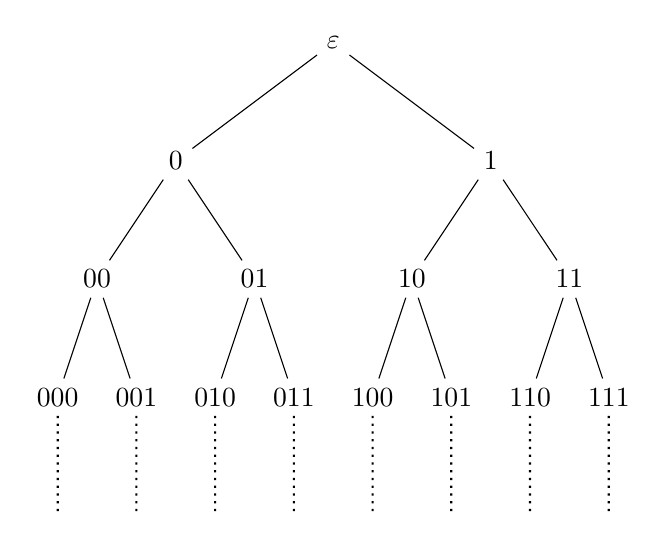
\begin{tikzpicture}[level 1/.style={sibling distance = 40mm}, 
                            level 2/.style={sibling distance = 20mm},
                            level 3/.style={sibling distance = 10mm}]
                \node {$\varepsilon$}
                    child {node {0}
                        child {node {00}
                            child {node {000}
                                child {edge from parent[dotted,thick]}
                            }
                            child {node {001}
                                child {edge from parent[dotted,thick]}
                            }
                        }
                        child {node {01}
                            child {node {010}
                                child {edge from parent[dotted,thick]}
                            }
                            child {node {011}
                                child {edge from parent[dotted,thick]}
                            }
                        }
                    }
                    child {node {1}
                        child {node {10}
                            child {node {100}
                                child {edge from parent[dotted,thick]}
                            }
                            child {node {101}
                                child {edge from parent[dotted,thick]}
                            }
                        }
                        child {node {11}
                            child {node {110}
                                child {edge from parent[dotted,thick]}
                            }
                            child {node {111}
                                child {edge from parent[dotted,thick]}
                            }
                        }
                    };
            \end{tikzpicture}
            \caption{The infinite tree $\mathcal{T}$}
            \label{fig:infinite_rooted_binary_tree}
        \end{figure}

        
        \begin{comment}
        HI TILLMAN!
        
        HI How's it going?
        
        All good.  We are all either editing or coding.
        Home safely?
        
        
        Yeah got there ok, I'm looking at the corrections for the algorithm.
        I can't stay for long so I'll have another look later on.
        
        No worries.  We are just slowly plugging away.
        
        Changing all references to the tree as $n$-ary.  Will restrict to n=2 for applications to F T V later.
        
        
        That sounds like a good plan, good luck!
        
        Cheers!
        \end{comment}
        
    Note that with this visualisation, the relation $\preceq$ determines an \emph{ancestor--descendant} relation on the vertices $\xns$.  Suppose $t$, $u$, $v$, and $w\in \xns$.  If $v\preceq w$ we say that $v$ is an \emph{ancestor of $w$} and that \emph{$w$ is a descendant of $v$}.  Further, if $v$ is an ancestor of $w$ and $|w|=|v| - 1$ we say that $w$ is a \emph{child of $v$} and that \emph{$v$ is the parent of $w$} (note that any vertex has at most one parent).  If $u$ and $v$ are both children of $t\in\xns$, then we say that $u$ and $v$ are \emph{siblings}.    
        
        
            \begin{definition}[Caret]
            For any word $ w $ in $\tn$, define $\wh{ w }$ to be the sub-tree of $\tn$ spanned by the set of vertices $ \{w\}\cup\{wx\mid x\in\xn\}$. We call $\wh{w}$ the \textit{($n$-ary) caret rooted at $ w $.}
            \end{definition}



When we refer to a sub-tree in $\tn$, we will always mean a tree which admits a decomposition as a union of $n$-ary carets.  We define such sub-trees below.

\begin{definition}[Full subtree] We say that a sub-tree $\mathcal{D}$ of $\tn$ is a \textit{full} sub-tree of $\tn$ if there is a set $C(\mathcal{D})\subset\xns$ so that for any edge $e$ of $\mathcal{D}$ there is $w_e\in C(\mathcal{D})$ so that $e$ is an edge of $\wh{w_e}$, and, for each $w\in C(\mathcal{D})$ the caret $\wh{w}$ is contained in $\mathcal{D}$.
\end{definition}

        
        \begin{definition}[Root of sub-tree]\label{def:root}
            Let $\D$ be any full non-empty sub-tree of $\tn$. Assign the \textit{root} of $\D$ be the vertex in $\D$ with the shortest length as a word in $\xns$.
        \end{definition}
            The above definition is well-defined since a sub-tree of $\tn$ must be connected, and having two distinct shortest words would imply some common descendant of these, but each vertex has at most one parent.
                    
        
        \begin{definition}[Leaf set]
            For any full non-empty sub-tree $\D$ of $\tn$, define the \textit{leaf set} $L_\D$ to be the set of all vertices of $\D$ with degree one.
        \end{definition}
        
            Note that for $w\in X_2^*$ the root of $\wh{ w }$ is $ w $ and we have $L_{\wh{ w }}=\{ w 0, w 1\}$.  We may visualise this as in Figure \ref{fig:caret}.

        \begin{figure}[h]\label{fig:caret}
            \centering
            
            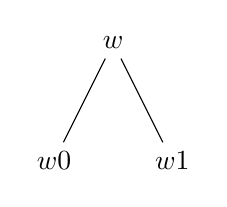
\begin{tikzpicture}
                \node {$ w $}
                    child {node {$ w  0$} }
                    child {node {$ w  1$} };
            \end{tikzpicture}
            \caption{A caret $\wh{ w }$ within $\T_2$}
            \label{fig:caret}
        \end{figure}
        
        \begin{definition}[Lower sub-tree]
            Let $ w $ be any vertex of $\tn$. Define its \textit{lower sub-tree} $\T_{ [w] }$ to be the sub-tree of $\tn$ spanned by the vertex set: $$V(\T_{ [w] } )\seteq\{ v \ \mid\  v \in\T\text{ and } w \preceq v \}.$$
        \end{definition}
        
        \begin{figure}[h]
            \centering
            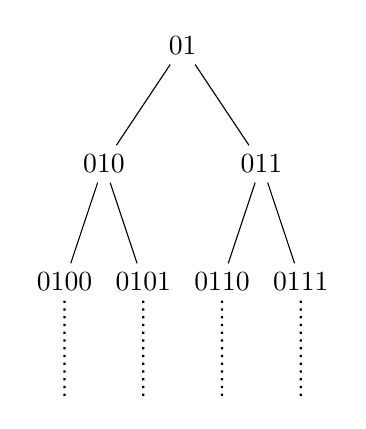
\begin{tikzpicture}[level 1/.style={sibling distance = 20mm}, 
                                    level 2/.style={sibling distance = 10mm},
                                    level 3/.style={sibling distance = 5mm},
                                    level 4/.style={sibling distance = 5mm}]
                \node {01}
                    child {node {010} 
                        child {node {0100}
                            child {edge from parent[dotted,thick]}
                        }
                        child {node {0101}
                            child {edge from parent[dotted,thick]}
                        }
                    }
                    child {node {011}
                        child {node {0110} 
                            child {edge from parent[dotted,thick]}
                        }
                        child {node {0111}
                            child {edge from parent[dotted,thick]}      
                        }
                    };
                \end{tikzpicture}
                \caption{The infinite lower sub-tree $\T_{[01]}$}
                \label{fig:lower-sub-tree}
        \end{figure}
        
        \begin{remark}
            It follows from this definition that for two incomparable vertices $ w , v $ in $\tn$, we have that $V(\T_{ [w] })\cap V(\T_{ [v] })=\varnothing$.
        \end{remark}
        
        \begin{definition}
            Let $w\in\xns$.  We set the \emph{boundary of $\T_{[w]}$} to be the set $w\Cn\subset \Cn$.
        \end{definition}
        
        \begin{definition}[Unions and intersections]
            Let $\R$ and $\s$ be full sub-trees of $\tn$. We define the following as subgraphs of $\tn$ spanned by these vertex sets:
            \begin{itemize}
                \item $\R\cup\s$ has vertex set $V(\R)\cup V(\s)$
                \item $\R\cap\s$ has vertex set $V(\R)\cap V(\s)$
            \end{itemize}
        \end{definition}
        
        \begin{definition}[Subtraction]
            Let $\R$ and $\s$ be any full sub-trees of $\tn$, and let $ w $ be the root of $\s$. If $\R$ and $\s$ satisfy the condition that $L_\s\subseteq L_\R$, then define $\R -\s$ to be the sub-tree of $\T$ spanned by the vertex set: $$V(\R -\s)\seteq (V(\R)\setminus V(\s))\cup \{ w \}.$$
        \end{definition}
        
        \begin{remark}
            The subtraction of full sub-trees can be thought of as taking a \textit{difference of carets} of the two trees. In other words, $\R-\s$ contains all the carets in $\R$ which are not present in $\s$.
        \end{remark}
        
        \begin{lemma}
        $\R$ and $\s$ be any full sub-trees of $\tn$ so that $L_\s\subseteq L_\R$.  Then, $\R-\s$ is the full subtree so that $C(\R-\s)=C(\R)\backslash C(\s)$. 
        \end{lemma}
        
        \begin{definition}[Corresponding sub-tree]
            Let $D=\{d_1, d_2, ..., d_k\}$ be a complete antichain of $\xns$, for some $k \in \mathbb{Z}_{>0}$. We call $\D$ the \textit{corresponding sub-tree} of $D$, and define it by the following: $$\D\seteq\T -\bigcup_{1\leq i\leq k} \T_{d_i}.$$
        \end{definition}
        
        Note that there is a natural bijection between complete antichains of $\xns$ and their corresponding trees.
        
        
        \begin{comment}
        \begin{definition}[Descendants]
            Let $w$ and $v$ be some vertices in $\T$. We say $v$ is a \textit{child} of $w$ if there exists some $x \in X$ such that $v=w x$. In this case we will denote $w$ to be a \textit{parent} of $v$. Also we say that all $v$ in $\T$ satisfying $w \prec v$ are \textit{descendants} of $w$, and all $y$ in $\T$ satisfying $y\prec w$ are \textit{ancestors} of $w$.
            
            Hence for any $w$, the caret $\wh{w}$ consists of $w$ and both of its children.
        \end{definition}
        \end{comment}
        
    \section{Definitions of $F$, $T$, and $V$}
    
        %Third rewrite
        
        In this section we will show how pairs of complete antichains of equal order can be used to define homeomorphisms of Cantor space. We will then use this to define Thompson's Group $V$, $T$, and $F$.
        
        \begin{definition}[Prefix exchange map]
        
            % R just a subset of Finite words
        
            Let $D$ be a complete antichain, $R \subseteq \CS$, and $\sigma: D \to R$ a map.  For each element $\rho \in \mathfrak{C}$ there exists unique $d \in D$ and $w \in \mathfrak{C}$ such that $\rho = d w$. Let $\varphi : \mathfrak{C} \to \mathfrak{C}$ be a function such that $$\rho \varphi = d  w  \varphi = d \sigma  w .$$ We call $\varphi$ the \textit{prefix exchange map} with respect to $\sigma$.
        
        \end{definition}
        
        We will justify the use of \textit{map} in this section, as at this point we only know that $\varphi$ is a set function and not a continous function between topological spaces. 
        
        \begin{theorem}\label{pem-cts}
            Prefix exchange maps are continuous.
        \end{theorem}
        
        \begin{proof}
        
            
        
            Let $D$ be a complete antichain, $R$ an antichain, $\sigma: D \to R$ a map, and $\varphi$ the prefix exchange map with respect to $\sigma$. We will show that $\varphi$ is continuous by showing that the preimage of every open set in $\CS$ is open.  We will do this by showing the pre-image of any cone is a union of cones.
            
            Let $w\in\{0,1,\ldots, n-1\}^*$.  We will show that  $w\Cn\varphi^{-1}$ is a union of cones.
            
            For each $d \in D$, we will consider $d\sigma$. If $d\sigma$ is incomparable to $w$, then the cone under $d$ will not be in $w\Cn\varphi^{-1}$. If $w \preceq d\sigma$, then $d\CS$ is in $w\Cn\varphi^{-1}$. Finally, if $d\sigma \prec w$, then we can find a $\Gamma \in X_n^*$ such that $d\sigma\Gamma = w$, and then $d\CS \cap w\Cn\varphi^{-1} = d\Gamma\CS$. In each of these cases, let the resulting open set be called $U_{w,d}$. 
            
            Now, it follows by construction that $w\Cn\varphi^{-1} = \bigcup_{d \in D}U_{w,d}$, which is the union of open sets and hence open.
            
            \begin{comment}
            
            Let $U$ be an open set of $\CS$ and $U'$ the open set $U \cap (\bigcup_{r \in R} r\CS$). If $U'=\emptyset$, then the preimage of $U$ is the empty set, which is open.
            
            Assume that $U' \neq \emptyset$. From Lemma \ref{union-open-cones}, we can find an index set $I$ and words $w_i \in \xns$ for all $i \in I$ such that $|w_i| \geq \text{ NOOOOO ANTICHAINS CAN BE INFINITE}$. $$U' = \bigcup_{i \in I}w_i \CS.$$ Since $U' \subseteq \bigcup_{r \in R} r\CS$, for each $w_i$ we can find $r_i \in R,w_i' \in \xns$ such that $w_i = r_iw_i'$. Now, $$U' \varphi^{-1} = \bigcup_{i \in I} w_i \CS = \bigcup_{i \in I}r_iw_i'\CS = \bigcup_{i \in I} r_i \sigma^{-1} w_i' \CS,$$ a union of elements from the basis $\mathscr{B}$. This proves that $U'\varphi^{-1}$, and therefore $U \varphi^{-1}$, is open.
            
            %add that phi inverse U' is phi inverse U
            
            \end{comment}
        \end{proof}
        
        \begin{comment}
        
        We will now define a map $\Phi$ which will allow us to define $V$. Let $D$ and $R$ be two complete antichains of the same order and consider a bijection $\sigma$ between them. We define $\Phi$ to be the prefix exchange map with respect to $\sigma$.
        
        \end{comment}
        
        Let $\sigma$ be a bijection between any two complete antichains $D$ and $R$. We'll denote by $\Phi_\sigma$ the prefix exchange map with respect to $\sigma$. 
        
        \begin{lemma}\label{phi-bijection}
        
            If $\sigma: D \to R$ is a bijection between two complete antichains, then $\Phi_\sigma$ is a bijection.
        \end{lemma}
        
        \begin{proof}
        
            
            Let $\sigma:D\to R$ be a bijection between two complete antichains. To prove $\Phi_\sigma$ is bijective we will show that $\Phi_\sigma$ is surjective and injective.
            
            Let $\rho \in \Cn$. Since $R$ is a complete antichain, there exists $r \in R$ and a $\omega \in \Cn$ such that $\rho = r \omega$. As $\sigma$ is a bijection, there exists $d \in D$ such that $d \sigma = r$. Hence $\rho = r \omega = d \sigma \omega = d \omega \Phi_\sigma$. As $\rho$ was arbitrary, $\Phi_\sigma$ is surjective.
            
            Now, let $\mu,\nu \in \Cn$ be two distinct elements in the domain. There exists $d_1,d_2 \in D$ and $\omega_1,\omega_2 \in \Cn$ such that $\mu = d_1 \omega_1$ and $\nu = d_2 \omega_2$. If $d_1 = d_2$, then $\omega_1 \neq \omega_2$ and $d_1 \sigma = d_2 \sigma$, so $d_1 \sigma \omega_1 \neq d_2 \sigma \omega_2 \Rightarrow \mu \Phi_\sigma \neq \nu \Phi_\sigma$. If $d_1 \neq d_2$, then $d_1 \sigma \neq d_2 \sigma$ and hence $d_1 \sigma \omega_1 \neq d_2 \sigma \omega_2 \Rightarrow \mu \Phi_\sigma \neq \nu \Phi_\sigma$. Therefore $\Phi_\sigma$ is also injective. 
            
            %better to use other 'definiton' of injectve, standard to set theory
                
        \end{proof}
        
        Since $\Phi_\sigma$ is a bijection, it has a well-defined inverse $\Phi_\sigma^{-1}$.
        
        \begin{lemma}\label{phi-inverse-pem}
            If $\sigma: D \to R$ is a bijection between two complete antichains, then:
            
            \begin{itemize}
                \item $\Phi_\sigma^{-1}$ is a prefix exchange map;
                \item $\Phi_\sigma$ is a homeomorphism; and
                \item $\Phi_\sigma^{-1}=\Phi_{\sigma^{-1}}$.
            \end{itemize}
            
        \end{lemma}
        
        \begin{proof}
            Let $\rho \in \mathfrak{C}_n$ with $\rho = r  \omega $ where $r \in R$ and $ \omega  \in \mathfrak{C}_n$. Then $$\rho\Phi_\sigma^{-1} = r \omega  \Phi_\sigma^{-1} = r \sigma^{-1}  \omega .$$ Therefore $\Phi_\sigma^{-1}=\Phi_{\sigma^{-1}}$ is a prefix exchange map. All three points follow from this.
        \end{proof}
        
        
        \begin{comment}
        \begin{cor}\label{phi-homeo}
            If $\sigma: D \to R$ is a bijection between two complete antichains then the mapping $\Phi_\sigma$ is a homeomorphism.
        \end{cor}
        \begin{proof}
            From Lemma \ref{phi-bijection}, \ref{phi-inverse-pem}, and Theorem \ref{pem-cts}, $\Phi$ is a homeomorphism.  
        \end{proof}
        \begin{cor}\label{phi-homeo}
            If $\sigma: D \to R$ is a bijection between two complete antichains then the mapping $\Phi_\sigma^{-1}=\Phi_{\sigma^{-1}}$.
        \end{cor}
        \end{comment}

        
        Let $V$ be the set of all prefix exchange maps with respect to bijections between two complete antichains. We will show that $V$ forms a group.
        
        The following lemma is a useful tool to prove that $V$ is closed under composition of maps.
        
        \begin{lemma}\label{union-open-cones}
            Let $n \in \mathbb{N}$ be given. Every open set $U$ of $\mathfrak{C}$ can be written as a union of clopen cones $w_i \mathfrak{C}$ such that $\forall i \in I , \  |w_i| > n$ where $w_i \in \xns$ and $I$ is some index set.
        \end{lemma}
        
        \begin{proof}
            Recall that $\mathscr{B} = \{w \mathfrak{C} : w \in X^*\}$ is a basis for Cantor space. Hence we can find an index set $I$ and words $w_i \in \xns$ such that $U = \bigcup_{i \in I} w_i \mathfrak{C}$. %add what we're going to do here
            If $|w_i| \leq n$, let $A_i = \{w_i v : v \in X^* \text{ and } |v|= n-|w_i|+1\}$ or $A_i= \{w_i\}$ otherwise. For each $i$, $w_i \mathfrak{C} = \bigcup_{a \in A_i}a \mathfrak{C}$. Therefore $$U = \bigcup_{i \in I} \bigcup_{a \in A_i} a \mathfrak{C}.$$ This proves the lemma.
        \end{proof}
        
        \begin{lemma}\label{comp-v-closed}
            Composition under $V$ is closed.
        \end{lemma}
        
        We will prove this using an algorithm. 
        
        \begin{algorithm}\label{composition-of-v-algorithm}
            Let $\Omega$ and $\Psi$ be two prefix exchange maps with respect to bijections $\pi : D \to R$ and $\tau : D' \to R'$, where $D$, $R$, $D'$, and $R'$ are all complete antichains. If $R = D'$, then $\Omega \Psi$ is a prefix exchange map with respect to the bijection $\pi \tau$, and hence is in $V$. Assume that $R \neq D'$. Let $\lambda$ be a map which we will define in the algorithm.
              
            \begin{enumerate}[label=Step \arabic*:]
                \item If $R \setminus D' = \emptyset$, go to \ref{r-minus-d-empty}. Otherwise, choose a $r \in R \setminus D'$. If $r \prec d'$ for some $d \in D'$, continue to \ref{r-prefix}. Otherwise, $d' \prec r$ for a unique $d' \in D'$, and continue to \ref{d-prefix}.
                
                \item\label{r-prefix} Let $A = \{d' \in D' : r \prec d'\}$ and $R'' = A \cup R \setminus \{r\}$. Let $B = \{r\pi^{-1}w : d' = rw \text{ for some } d' \in A \text{ and } w \in X^*\}$ and $D'' = D \cup B \setminus \{r\pi^{-1}\}$. For each $b \in B$, we can find a $w_b \in \xns$ such that $r\pi^{-1}w_b = b$. Define $b\lambda=r w_b \tau$ for each $b \in B$. 
                
                Set $R'' = R$ and $D'' = D'$. Return to Step 1.
                
                \item\label{d-prefix} Let $A = \{r \in R : d' \prec r\}$ and $D'' = D' \cup A \setminus \{d'\}$. Let $B = \{d'\tau w : r = d'w \text{ for some } w \in X^*\}$. Let $R'' = R' \cup B \setminus \{d'\tau\}$. For each $a \in A$, we can find a $w_a \in \xns$ such that $r = d'w_a$. Define $a\pi^{-1} \lambda = d'\tau w_a$ for each $a \in A$.
                
                Set $R'' = R'$ and $D'' = D'$. Return to Step 1.
                
                \item\label{r-minus-d-empty} If $D' \setminus R = \emptyset$, go to \ref{final-step}. Otherwise, choose a $d' \in D' \setminus R$. If $d' \prec r$ for some $r \in R$, continue to \ref{d'-prefix}. Otherwise, $r \prec d'$ for a unique $r \in R$, and continue to \ref{r-prefix-2}.
                
                \item\label{d'-prefix} Let $A = \{r \in R : d' \prec r\}$ and $D'' = D' \cup A \setminus \{d'\}$. Let $B = \{d' \tau w : r = d'w \text{ for some } w \in X^*\}$. Let $R'' = R' \cup B \setminus \{d'\tau\}$. For each $a \in A$, we can find a $w_a \in \xns$
                such that $r = d'w_a$. Define $a\pi^{-1}\lambda = d'\tau w_a$ for each $a \in A$.
                
                Set $R'' = R'$ and $D'' = D'$. Return to Step 1.
                
                
                \item\label{r-prefix-2} Let $A = \{d' \in D : r \prec d'\}$ and $R'' = A \cup R \setminus \{r\}$. Let $B = \{r\pi{-1} w : d' = rw \text{ for some } d' \in A \text{ and } w \in X^*\}$ and $D'' = D \cup B \setminus \{r \pi^{-1}\}$. For each $b \in B$, we can find a $w_b \in \xns$ such that $r \pi^{-1} w_b = b$. Define $b \lambda rw_b \tau$ for each $b \in B$.
                
                Set $R'' = R$ and $D'' = D'$. Return to Step 1.
                
                \item\label{final-step} For each $x \in R \cap D'$, define $x\pi^{-1} \lambda = x\tau$. This is the end of the algorithm.
            \end{enumerate}
              
        \end{algorithm}
        
        \begin{lemma}\label{lambda-bijection}
            Let $\Omega$, $\Psi$, $D$, $R$, $D'$, $R'$, $\pi$, and $\tau$ be like they are in algorithm \ref{composition-of-v-algorithm}. The sets generated in this algorithm are complete antichains and the map $\lambda$ is a bijection. Furthermore, the prefix exchange map with respect to $\lambda$ is equivalent to the homeomorphism $\Omega\Psi$.
        \end{lemma}
        
        \begin{proof}
            Later...
        \end{proof}
        
        We can now prove lemma $\ref{comp-v-closed}$.
        
        \begin{proof}[Proof of lemma \ref{comp-v-closed}]
            From Algorithm \ref{composition-of-v-algorithm} and lemma \ref{lambda-bijection}, for every prefix exchange map $\Omega$ and $\Psi$ with respect to bijections $\pi : D \to R$ and $\tau : D' \to R'$ respectively, we can find complete antichains $Q$ and $W$ and a bijection $\lambda : Q \to W$ such that $\Omega\Psi$ is a prefix exchange map with respect to $\lambda$. 
        \end{proof}
        
        \begin{lemma}
            The set $V$ is a group under composition of functions.
        \end{lemma}
        
        \begin{proof}

            From lemma \ref{comp-v-closed}, $V$ is closed under composition of functions. The prefix exchange map with respect to the identity mapping of a complete antichain is the identity homeomorphism. The composition of functions is associative.
            
            Let $\Theta$ be a prefix exchange map in $V$. An identical argument as in lemma \ref{phi-inverse-pem} shows that that $\Theta^{-1}$ is a prefix exchange map. Therefore every element in $V$ has an inverse.
            
            This concludes the proof that $V$ is a group.
           
        \end{proof}
        
        We are now in a position to define the Thompson's Groups.
        
        \begin{definition}[Thompson's Groups]\label{thompsons-groups}
            
            Let $\Psi$ be a prefix exchange map with respect to the bijection $\pi : D \to R$, where $D$ and $R$ are complete antichains. Suppose that $D = \{d_1,d_2,...,d_n\}$ and $R=\{r_1,r_2,...,r_n\}$ are in lexicographic order. Let $F$ and $T$ be subsets of $V$, defined below.
            
            \begin{itemize}
                \item The group $V$ is called \textit{Thompson's Group $V$}.
                \item If $\forall \ 1 \leq i \leq n$, $d_i \pi = r_i$, then let $\Psi \in F$. All elements in $F$ are of this form. We call $F$ \textit{Thompson's Group $F$.}
                \item If $\forall \ 1 \leq i \leq n$, $d_i \pi = r_{i \mod{n}}$, then let $\Psi \in T$. All elements in $T$ are of this form. We call $T$ \textit{Thompson's Group $T$.}
            \end{itemize}
            
        \end{definition}
        
        From the definition we can see that $F \subseteq T \subseteq V$. As expected from their names, it can be shown that $F$ and $T$ are subgroups of $V$.
        
    \section{Tree Pairs}
    
        We will now give a way to represent elements of $V$ using objects called tree pairs. 
        
        \begin{definition}[Tree Pair]
            Let $D$ and $R$ be two complete antichains of equal order and $\sigma$ a bijection between them. We define the triple $(\D,\R,\sigma)$ to be a \textit{tree pair} where $\D$ and $\R$ are the corresponding trees of $D$ and $R$ respectively.
        \end{definition}
        
        For a tree pair $(\D,\R,\sigma)$, the sets $L_\D$ and $L_\R$ are complete antichains. Since $\sigma$ is a bijection between them, this defines a prefix exchange map with respect to $\sigma$. In Corollary \ref{phi-homeo}, we showed that this prefix exchange map is a homeomorphism of Cantor space and from Definition \ref{thompsons-groups}, an element of Thompson's Group $V$. Therefore, every tree pair represents an element of $V$. Conversely, if an element of $V$, say $\Phi$, is a prefix exchange map with respect to $\sigma : D \to R$, then the tree pair $(\D,\R,\sigma)$ is a representation of this element.
        
        \begin{remark}\label{not-unique-tree-pair}
            There is not a unique tree pair for each element in $V$, but every tree pair represents a unique element of $V$, as we will show in the next subsection.
        \end{remark}
        
        \subsection{Altering tree pairs}
            
            In this subsection, we will show different ways of altering tree pairs so they represent the same element of $V$.
        
        \begin{comment} %second rewrite
        In this section we will define Thompson's Groups using tree pairs. Before this however, we will show how pairs of complete antichains of equal order can be used to define homeomorphisms of the Cantor set.
        
        Let $D$ and $R$ be two complete antichains of order $n \in \mathbb{N}$ and let $\sigma$ be a bijection between them. We'll show that $\sigma$ induces a homeomorphism of $\mathfrak{C}$.
        
        Let $p \in \mathfrak{C}$. Since $D$ is a complete antichain, $\exists ! d \in D$ and $ w  \in \mathfrak{C}$ such that $p = d  w $. Let $\Phi$ be the mapping $$p \Phi = d  w  \Phi = d \sigma  w .$$
        
        \begin{claim}
            The mapping $\Phi$ is a bijection.
        \end{claim}
        
        \begin{proof}
            Let $p \in \mathfrak{C}$ and write it as $p = r  w $ for some $r \in R$ and $ w  \in \mathfrak{C}$. Since $\sigma$ is a bijection, $\Phi$ has the natural inverse described by $$p \Phi^{-1} = r  w  \Phi^{-1} = r \sigma^{-1}  w .$$ Hence $\Phi$ is a bijection. 
        \end{proof}
        
        All that's left is to show is that $\Phi$ and $\Phi^{-1}$ are continuous.
        
        
        \begin{claim}
            Let $n \in \mathbb{N}$ be given. Every open set $U$ of $\mathfrak{C}$ can be written as a union of clopen cones $\alpha_i \mathfrak{C}$ such that $\forall i , \ \mid\alpha_i\mid > \midn\mid$ where $\alpha_i \in \xns$ and $I$ is some index set.
        \end{claim}
        
        \begin{proof}
        
        \end{proof}
        
        Let $U$ be some open set of $\mathfrak{C}$. From the claim, we can find an index set $I$ such that $$U = \bigcup_{i \in I} \alpha_i \mathfrak{C}.$$ For each $\alpha_i \in \xns$, there are unique words $r_i \in R$ and $w_i \in \xns$ such that $\alpha_i = r_i w_i$. Now, $$U \Phi^{-1} = (\bigcup_{i \in I} \alpha_i \mathfrak{C}) \Phi^{-1} = (\bigcup_{i \in I} r_i w_i \mathfrak{C}) \Phi^{-1} = \bigcup_{i \in I} r_i \sigma^{-1} w_i \mathfrak{C}.$$ This shows that the preimage of any open set in $\mathfrak{C}$ is the union of clopen cones and hence is also open. Therefore $\Phi$ is continuous. A similar argument shows that $\Phi^{-1}$ is continuous, which means $\Phi$ is a homeomorphism.
        
        Homeomorphisms arising this way form a group under composition: Thompson's Group $V$.
        \end{comment}
        
        
        \begin{comment}
        In this section we will define Thompson's Group using tree pairs. Before this however, we will show how antichains can be used to define homeomorphisms of the Cantor set.
        
        Suppose that $D = \{d_1,...,d_k\}$ and $R = \{r_1,...,r_k\}$ are two complete antichains of order $k \in \mathbb{Z}_{>0}$. Let $\sigma$ be a bijection between $D$ and $R$ that maps each word $d_i$ to $r_j$ ($1 \leq i,j \leq j$). We will now show that $\sigma$ induces a homeomorphism $\Phi$ of $\mathfrak{C}$. Let $ w  \in \mathfrak{C}$ and let $d_i$ be the unique element in $D$ such that $ w  = d_i  v $ for some $ v  \in X^ w $. The map $\Phi$ then acts on $ w $ by $$ w  \Phi = d_i  v  \Phi = d_i \sigma  v  = r_j  v .$$ It's clear that $\Phi$ is a bijection of $\mathfrak{C}$, so all that's left to show is continuity of $\Phi$ and $\Phi^{-1}$. 
        
        Suppose that $V$ is some open subset of $\mathfrak{C}$. Then since the set of clopen cones $\mathscr{B}$ form a basis of $\mathfrak{C}$, there exists an index set $I$ such that $V = \bigcup_{t \in I} \alpha_t \mathfrak{C}$ where each $\alpha_t \mathfrak{C}$ is a subset of some unique clopen cone $r_{i_t} \mathfrak{C} \ (1 \leq i_t \leq k)$. Therefore $\forall t \in I \ \exists w_t \in \xns$ such that $\alpha_t = r_{i_t}w_t$. Finally, $$V\Phi^{-1} = (\bigcup_{t \in I} \alpha_t \mathfrak{C}) \Phi^{-1} = \bigcup_{t \in I} r_{i_t}\sigma^{-1}w_t \mathfrak{C}.$$ Hence $V\Phi^{-1}$ is the union of clopen cones and is therefore also open. Continuity of $\Phi^{-1}$ follows from a similar argument and proves that $\Phi$ is a homeomorphism of $\mathfrak{C}$.
        
        The homeomorphisms of $\mathfrak{C}$ which arise from a bijection between two complete antichains described above form a group: Thompson's Group $V$. We will now define tree pairs which are used to represent elements from $V$.

        \begin{definition}[Tree Pair]
            Let $D$ and $R$ be two complete antichains of equal order and $\sigma$ a bijection between them. We define the triple $(\D,\R,\sigma)$ to be a \textit{tree pair} where $\D$ and $\R$ are the corresponding trees of $D$ and $R$ respectively.
        \end{definition}
        
        \end{comment}
        
        \begin{comment}
            We will now show that tree pairs represent a bijection of the Cantor set. Let $(D,R,\sigma)$ be a tree pair and $p \in \mathfrak{C}$. Suppose that $L_D = \{d_1,d_2,...,d_k\}$ and $L_R = \{r_1,r_2,...,r_k\}$. Since $L_D$ is a complete antichain, there exists a unique $d_i \in L_D$ ($1 \leq i \leq k$) and some $x \in \mathfrak{C}$ such that $p = d_ix$. It's clear that the mapping $p \mapsto r_{i\sigma}x$ is a bijection of Cantor space. We define Thompson's Group $V$ to be the group of these bijections with composition and we define $F$ and $T$ in terms of $\sigma$:
        
        
        
        \begin{itemize}
            \item If $t\sigma = t+n \mod k$ ($1 \leq t \leq k$, $n \in \mathbb{Z}$) then $(D,R,\sigma)$ represents an element of $T$.
            \item  If $j\sigma = j$ ($1 \leq j \leq k$) then $(D,R,\sigma)$ represents an element of $F$.
        \end{itemize}
        \end{comment}
        
        \begin{definition}[Pair of dangling carets]\label{pair-of-dangling-carets}
            \begin{comment}
                Let $(\D,\R,\sigma)$ be a tree pair of some element $\alpha \in V$. Consider some carets $\wh{A}$ of $\D$ rooted at $a \in \{0,1\}^*$ and $\wh{B}$ of $\R$ rooted at $b \in \{0,1\}^*$ with $a0,a1 \in L_\D$ and $b0,b1 \in L_\R$ of $\D$ and $\R$ respectively for some $a,b \in \{0,1\}^*$. We call $(\wh{A},\wh{B})$ \textit{dangling carets} of $(\D,\R,\sigma)$ if $(a0) \sigma = b0$ and $(a1) \sigma = b1$.
            \end{comment}
        
            % rewrite of above
            Let $(\D,\R,\sigma)$ be a tree pair representing some element $\alpha \in V$. Consider some carets $\wh{a}$ and $\wh{b}$ such that $L_{\wh{a}} \subseteq L_\D$ and $L_{\wh{b}} \subseteq L_\R$. We call $(\wh{a},\wh{b})$ a \textit{pair of dangling carets} of $(\D,\R,\sigma)$ if $(a0) \sigma = b0$ and $(a1) \sigma = b1$.
        \end{definition}
        
        \begin{lemma}\label{dangling-carets-delete-same-element}
            Consider a tree pair $(\D,\R,\sigma)$ representing an element $\alpha \in V$ with a pair of dangling carets $(\wh{a},\wh{b})$. Then the tree pair $(\D - \wh{a}, \R - \wh{b}, \sigma')$, where $$d \sigma' = \begin{cases} d \sigma \quad & \text{if } d \neq a \\ b \quad & \text{if } d=a \end{cases}$$ for all $d \in L_\D$, represents the same element $\alpha$. 
        \end{lemma}
        
        \begin{proof}
            Let $\Psi$ be the prefix exchange map with respect to $\sigma: L_\D \to L_\R$ and $\Omega$ be the prefix exchange map with respect to $\sigma: L_{\D'} \to L_{\R'}$. Consider an element $\rho \in \CS$. If $a \nprec \rho$, then $\rho \Psi = \rho \Omega$. Otherwise, either $a0 \prec \rho$ or $a1 \prec \rho$. Suppose $a0 \prec \rho$, and let $\omega \in \CS$ such that $\rho = a0\omega$. Then $$\rho \Psi = a0\omega \Psi = a0 \sigma \omega = b0 \omega = a \sigma' 0 \omega = \rho \Omega$$ and a similar argument shows the same if $a1 \prec \rho$. Hence $\Psi = \Omega$.
        \end{proof}
    
        \begin{algorithm}[Minimisation]\label{minimisation}

            Let $(\D,\R,\sigma)$ be a tree pair representing an element $\alpha$ in $V$. 
    
            \begin{enumerate}[label=Step \arabic*:]
            
                \item Let $\D' \seteq \D$, $\R' \seteq \R$, and $\sigma \seteq \sigma'$.
            
                \item If the tree pair $(\D', \R', \sigma')$ has no dangling carets, then terminate. Otherwise, choose dangling carets $(\wh{a},\wh{b})$ and go to Step 2.
        
                \item Let $\D''\seteq\D' -\wh{a}$, $\R''\seteq\R' -\wh{b}$. Define $\sigma'':\D' \rightarrow\R'$ by:
                $$d \sigma'' = \begin{cases} d\sigma \quad &\text{if } d \neq a \\ b \quad &\text{if } d=a \end{cases}$$ for all $d\in\D''$. Let $\D' = \D''$, $\R' = \R''$, and $\sigma' = \sigma''$ and return to Step 2. 
        
            \end{enumerate}
            
            We call the tree pair $(\D', \R', \sigma')$ a \textit{reduced tree pair} of $(\D,\R,\sigma)$.
            
        \end{algorithm}
        
        Since there are finite edges in a any tree pair, Algorithm \ref{minimisation} must terminate.
        
        \begin{remark}
            It can be shown that there is a unique reduced tree pair for every tree pair, and hence the choice of dangling carets in Step 2 of Algorithm \ref{minimisation} does not matter. CITE EWA.
        \end{remark}
        
        \begin{lemma}
            Let $(\D,\R,\sigma)$ be a tree pair representing an element $\alpha \in V$. Then the reduced tree pair $(\D',\R',\sigma')$ of $(\D,\R,\sigma)$ represents the same element $\alpha$.
        \end{lemma}
        
        \begin{proof}
            This follows from repeated application of Lemma \ref{dangling-carets-delete-same-element}.
        \end{proof}
        
        We can also add dangling carets to tree pairs, which will be important later.
    
        \begin{definition}[Adding a caret]\label{adding-a-caret}
        
            Let $(\D,\R,\sigma)$ be a tree pair representing an element $\alpha \in V$ and consider $d \in L_\D$. Let $\D' = \D \cup \wh{d}$,  $\R' = \R \cup \wh{d\sigma}$, and define $\sigma'$ to be the map $$l\sigma' = \begin{cases} l\sigma \quad &\text{if } l \notin \{d0,d1\} \\ r0 \quad &\text{if } l=d0  \\ r1 \quad &\text{if } l = d1 \end{cases}$$ for all $l \in L_{\D'}$. We say that we've \textit{added a caret to $d$}.
    
    \end{definition}
    
    \begin{lemma}
        Let $(\D,\R,\sigma)$ be a tree pair representing an element $\alpha \in V$ and consider $d \in L_\D$. The tree pair $(\D',\R',\sigma')$ resulting from adding a caret to $d$ as in Definition \ref{adding-a-caret} represents the same element $\alpha$.
    \end{lemma}
    
    \begin{proof}
        From the definition, $(\wh{d}, \wh{d\sigma'})$ is a dangling caret of $(\D',\R',\sigma')$. From Lemma \ref{dangling-carets-delete-same-element}, this represents the same element as $(\D,\R,\sigma)$.
    \end{proof}
    
    %below here define expansion as adding a dangling caret to a tree pair
    
    All of the above justifies Remark \ref{not-unique-tree-pair}.
    
    \section{Chains}
    
        In this section we will define chains which will allow us to partition all the leaves in a tree pair.
        
        \begin{definition}[Chain]
            
            Consider $w \in X^*$, $\alpha \in V$, and a continuous subinterval $L \subseteq \mathbb{Z}$. Then the \textit{$L$ chain at $w$} is the sequence $(w\alpha^i)_{i \in L}$.
        
        \end{definition}
        
        \begin{definition}[Leaf chain]
            Let $(\D,\R,\sigma)$ be a tree pair representing an element $\alpha \in V$. Consider $l \in L_\D$. There exists a maximal $k \in \mathbb{Z}_{>0}$ such that
            
            \begin{itemize}
                \item for $0 \leq i < k$, $l \alpha^i \in L_\D$;
                \item for $0 < j \leq k$, $l \alpha^j \in L_\R$;
                \item for $0 \leq s,t < k$ and $s \neq t$, $l \alpha^s \neq l \alpha^t$.
            \end{itemize}
            Let $L=\{0,1,...,k\}$. We define the \textit{leaf chain at $l$} to be the $L$ chain at $l$.
        \end{definition}
        
        \begin{definition}[Complete leaf chain]
            Consider the leaf chain $(l\alpha^i)_{i=0}^k$ for some tree pair $(\D,\R,\sigma)$. We call this chain a \textit{complete leaf chain} if either $l \in L_\D \setminus L_\R$ and $l \in L_\R \setminus L_\D$, or $l = l \alpha^k$.
        \end{definition}
    
        \begin{remark}
            We will refer to leaf chains which are not complete as \textit{partial leaf chains}.
        \end{remark}
        
        We will apply an algorithm to classify complete leaf chains into exactly one of five types.
        
        \begin{algorithm}[Classifying complete leaf chains]
        \label{chain-classification}
            Consider a tree pair $(\D,\R,\sigma)$ representing an element $\alpha$ in $V$ and let $(l \alpha^i)_{i=0}^k$ be a complete leaf chain for this tree pair. 

            \begin{enumerate}[label=Step \arabic*:]
        
            \item If $l = l \alpha^k$ then we call it a \textit{$P$-chain}, for \textit{``periodic''} and terminate. Otherwise, continue to Step 2.
            \item If $l \prec l \alpha^k$ then we call it an \textit{$A$-chain}, for \textit{``attractor''} and terminate. Otherwise, continue to Step 3.
            \item If $l \alpha^k \prec l$ then we call it an \textit{$R$-chain} for \textit{``repeller''} and terminate. Otherwise, continue to Step 4.
            \item If $l \prec r$ for $r \in L_\R \setminus L_\D$ or $l \alpha^k \prec d$ for $d \in L_\D \setminus L_\R$, then we call it an \textit{$F$-chain} for \textit{``fragmenter''} and terminate. Otherwise, continue to Step 5.
            \item Call $(l\alpha)_{i=0}^k$ a \textit{$S$-chain} for \textit{``source-sink''}.
        
        \end{enumerate}
    \end{algorithm}    
    
    From this algorithm, every complete leaf chain is classified as exactly one chain type. We give names to the elements in a complete leaf chain:
    
    \begin{definition}[Leaves of complete leaf chains]\label{types-of-leaves}
    
        Let $(l \alpha^i)_{i=0}^k$ be a complete leaf chain for a tree pair $(\D,\R,\sigma)$. We call
    
        \begin{itemize}
        
            \item $l$ a \textit{repeller} of period $k$ and $l \alpha^k$ a \textit{range of repulsion} if $(l \alpha^i)_{i=0}^k$ is an $R$-chain;
            
            \item $l \alpha^k$ an \textit{attractor} of period $k$ and $l$ a \textit{domain of attraction} if $(l \alpha^i)_{i=0}^k$ is an $A$-chain;
            
            \item $l$ a \textit{source} and $l \alpha^k$ is a \textit{sink} if $(l \alpha^i)_{i=0}^k$ is a $S$-chain;
            
            \item $l$ a \textit{start-fragmenter} if $(l \alpha^i)_{i=0}^k$ is a $F$-chain and $l \prec r$ for $r \in L_\R \setminus L_\D$;
            \item $l\alpha^k$ a \textit{end-fragmenter} if $(l \alpha^i)_{i=0}^k$ is a $F$-chain and $l\alpha^k \prec d$ for $d \in L_\D \setminus L_\R$;
            
            \item leaves in $L_\D \cap L_\R$ \textit{neutral leaves}.
            
            
        \end{itemize}
    
    \end{definition}
    
    
    \begin{comment}
    
    \section{Leaves and Chains} 
    
        In this section we will define a finite sequence using tree pairs which we will call \textit{leaf chains}. These leaf chains and their types will be important in our algorithm in section \ref{slow-rollings}.
        
        \begin{definition}[Non-neutral Leaf Chain]
                Consider a tree pair $(\D,\R,\sigma)$ representing an element $\alpha$ of $V$. Consider a sequence $(l \alpha^i)_{i=0}^k$ for some leaf $l \in L_\D \setminus L_\R$ and some $k \in \mathbb{Z}_{>0}$ such that $l \in L_\D$, $l \alpha^j \in L_\D \cap L_\R \ (0 < j < k)$, and either $l \alpha^k \notin L_\D$ or $l \alpha^{k} = l$.
        \end{definition}
        
        \begin{definition}[Neutral Leaf Chain]
                Consider a tree pair $(\D,\R,\sigma)$ representing an element $\alpha$ of $V$. Consider a sequence $(l \alpha^i)_{i=0}^k$ for some leaf $l \in L_\D \cap L_\R$ and some $k \in \mathbb{N}, k > 0$ such that $l \in L_\D \cap L_\R,$ $l \alpha^j \in L_\D \cap L_\R \ (0 < j < k)$, and either $l \alpha^k \notin L_\D$ or $l \alpha^{k} = l$.
        \end{definition}
        
    % put example here :)
    
    We will now classify non-neutral leaf chains into 7 disjoint types.
    
    \begin{lemma}[Classifying types of non-neutral leaf chains]
        Let $(\D,\R,\sigma)$ be a tree pair representing an element $\alpha \in V$. Each leaf chain $(l\alpha^i)_{i=0}^k$ for some $l \in L_\D$ can be classified into exactly one type, by the procedure given below:
        
        \begin{algorithm} [Classifying non-neutral chains]
            The algorithm terminates when the chain is classified.
            \begin{enumerate}[label=Step \arabic*:]
                \item If $l\alpha^k \prec l$, then this is an \textit{$R$-chain};
                \item If $l \prec l\alpha^k$, then this is an \textit{$A$-chain}.
                \item If $l \alpha^k \prec x$ for some $x \in L_\D \setminus L_\R$ and $l \nprec y$ for any $y \in L_\R \setminus L_\D$, then this is an \textit{$EF$-chain}.
                \item If $l \prec y$ for some $y \in L_\R \setminus L_\D$ and $l \alpha^k \nprec x$ for some $x \in L_\D \setminus L_\R$, then this is an \textit{$SF$-chain}.
                \item If $l \alpha^k \prec x$ for some $x \in L_\D \setminus L_\R$ and $l \prec y$ for some $y \in L_\R \setminus L_\D$, this is an \textit{$SEF$-chain}.
                \item otherwise, we classify it as an \textit{$SS$-chain}.
                % \item We classify as \textit{$SS$-chain} otherwise.
                
            \end{enumerate}
        \end{algorithm}
    \end{lemma}
    % this is getting axed
    % \begin{definition}[Types of Leaf chains]
        
    %     Let $(\D,\R,\sigma)$ be a tree pair representing an element $\alpha \in V$ and suppose $(l\alpha^i)_{i=0}^k$ is a leaf chain for some $l \in L_\D$. We say $(l\alpha^i)_{i=0}^k$ is a:
        
    %     \begin{itemize}
    %         \item \textit{$R$-chain} if $l \alpha^k \prec l$;
            
    %         \item \textit{$A$-chain} if $l \prec l \alpha^k$;
            
    %         \item \textit{$EF$-chain} if  $l \alpha^k \prec x$ for some $x \in (L_\D \setminus L_\R) \setminus \{l\}$ and $l \nprec y$ for any $y \in (L_\R \setminus L_\D) \setminus \{l \alpha^k\}$;
            
    %         \item \textit{$SF$-chain} if $l \prec x$ for some $x \in (L_\R \setminus L_\D) \setminus \{l \alpha^k\}$ and $l \alpha^k \nprec y$ for any $y \in (L_\D \setminus L_\R) \setminus \{l\}$;
            
    %         \item \textit{$SEF$-chain} if $l \alpha^k \prec x$ for some $x \in (L_\D \setminus L_\R) \setminus \{l\}$ and $l \prec y$ for some $y \in (L_\R \setminus L_\D) \setminus \{l \alpha^k\}$;
            
    %         \item \textit{$P$-chain} if $l = l \alpha^k$;
            
    %         \item \textit{$SS$-chain} otherwise.
    %     \end{itemize}
    %     We call $P$-chains \textit{periodic leaf chains} and all other leaf chains \textit{non-periodic leaf chains}.
    
    % \end{definition}
    
    \begin{remark}[Classifying leaf chains in terms of each other]
    
        % here put the prefix of other chains definition thing for leaf chains since that's what we use in the algorithm
        Observe that the all the \textit{non-periodic leaf chains} generated from $L_\D$, must be generated only from $L_\D \setminus L_\R$.
        Let $(l \alpha^i)_{i=0}^k$ be a leaf chain. We can interpret the above like this:
        
        \begin{itemize}
        
            \item $EF$ or \textit{end fragmenter} chains: $(l\alpha^i)_{i=0}^k$ can be an $EF$-chain if $l \alpha^k \preceq y$ where $y$ is the first element of some \textit{non-periodic chain} other than $(l\alpha^i)_{i=0}^k$. 
            
            \item $SF$ or \textit{start fragmenter} chains:Similarly $(l\alpha^i)_{i=0}^k$ can be an $SF$-chain if $l \preceq x$ where $\xn$ is the last element of some \textit{non-periodic chain} other than $(l\alpha^i)_{i=0}^k$. 
            
            \item $SF$ or \textit{start-and-end fragmenter}. If both of them above are satisfied then it is an $SEF$-chain
        
        \end{itemize}
    \end{remark}
    
    % add an example explaining fragmentation
    

    
    \begin{definition}[Types of leaves]
    
        Let $(\D,\R,\sigma)$ be a tree pair and $(l \alpha^i)_{i=0}^k$ be a leaf chain, then we call
    
        \begin{itemize}
        
            \item $l$ a \textit{repeller} of period $k$ and $l \alpha^k$ a \textit{range of repulsion} if $(l \alpha^i)_{i=0}^k$ is an $R$-chain;
            
            \item $l \alpha^k$ an \textit{attractor} of period $k$ and $l$ a \textit{domain of attraction} if $(l \alpha^i)_{i=0}^k$ is an $A$-chain;
            
            \item $l$ a \textit{source} and $l \alpha^k$ is a \textit{sink} if $(l \alpha^i)_{i=0}^k$ is a $SS$-chain.
            
        \end{itemize}
        
        We call elements of $L_\D \cap L_\R$ \textit{neutral leaves}.
    
    \end{definition}

    \end{comment}
    
    
    \section{Revealing Pairs}

        It is possible to alter a tree pair $(\D,\R,\sigma)$ to $(\D',\R',\sigma')$ such that there are no complete leaf chains of type $F$ for $(\D',\R',\sigma')$. We give these types of altered trees a name:
        
        \begin{definition}[Revealing pair]
        \label{revealing-pair}
            A tree pair $(\D,\R, \sigma)$ is said to be a \emph{revealing pair} if all complete leaf chains are of type $P$, $R$, $A$, or $S$.
        \end{definition}
        
        Our algorithm in Section \ref{final-algorithm} outputs a revealing pair for any given tree pair. To understand the algorithm and form a termination algorithm for it, we will give a visual representation for the types of leaves defined in Definition \ref{types-of-leaves}, using tree pairs and connected components.
        
        \begin{definition}[Connected components]
            Let $S$ be a full subtree of $\tn$. We define an equivalence relation $\sim$ on $S$, such that for all $a,b \in X^*$  $a \sim b$ if and only if there exists a path from $a$ to $b$ in $S$. This is the standard definition of connectedness in graphs.
            
            We can define the connected components of $S$ as the subtrees of $\tn$ spanned by set of words in each equivalence class.
        \end{definition}
        
        \begin{definition}[Complementary Components]
            Let $(\D,\R, \sigma)$ be a tree pair of an element of V.
            
            A complementary component of $(\D,\R, \sigma)$ is a connected component of $\D-\R$ or $\R-\D$.
        \end{definition}
        
        % I think this needs to be a lemma that we prove or cite Ewa for. 
        % TODO
        \begin{lemma} Each connected component of a revealing pair contains exactly one attractor or repeller.

            \begin{proof}
        
            Let $(\D,\R, \sigma)$ be a tree pair of an element of V represented by $\alpha$.

            Proceeding by contradiction, assume that $\D - \R$ contains a connected component with atleast two distinct repellers. We shall name these $l_1, l_2$ such that $(l_1\alpha^i)_{i=0}^l$ and $(l_1\alpha^i)_{i=0}^l$ are R-chains. This is the case if and only if $l_1 \prec l_1\alpha^k$ and $l_2 \prec l_2\alpha^k$, but $l_1\alpha^k$ and $l_2\alpha^k$ must be leaves in $\R$, and the unique leaf in $\R$ such that it is the prefix of the leaves in our connected component is the root of the connected component. This implies $l_1\alpha^k = l_2\alpha^k$ which gives us $l_1 = l_2$ by invertibility of $\alpha^k$. By symmetry, as a repeller for $\alpha$ is an attractor for $\alpha^{-1}$, a connected component of a revealing tree pair cannot contain more than one repeller or attractor.

            Assuming that a connected component in $\D - \R$ does not contain a repeller. The root of this connected component is a leaf in $\R$, we name this $l$, which means there exists a leaf $l'$ and chain $(l'\alpha^i)_{i=0}^k$ such that $l$ is in this chain. $l$ is the root of a connected component, so it is not a sink. Therefore, this chain must be an $F-chain$, which contradicts that the pair is revealing.


            \end{proof}
        \end{lemma}
        

\begin{comment}

    The algorithm we will describe will take a tree pair of some element in $V$ and transform it into a revealing pair. We will take a tree pair $(\D,\R,\sigma)$ of some element $\alpha \in V$ and add carets to the leaves of the trees, determined by the algorithm until we have a revealing pair. We call this process "\textit{slow rollings}".
    
\end{comment}
\begin{comment} % this is done above now
    \begin{remark}
        Let $(D,R,\sigma)$ be a tree pair of some element $\alpha \in V$. If $(A,B)$ are dangling carets of $(\D,\R,\sigma)$ with roots $a,b \in \{0,1\}^*$ respectively, then $(\D-A, \R-B, \sigma')$ represents the same element $\alpha$ where, for any $l \in L_{D-A}$
        \begin{equation}
            \sigma'(l) = 
                \begin{cases}
                    \sigma(l) & \text{if } l \notin \{a,b\} \\
                    b & \text{if } l = a
                    
                \end{cases}
        \end{equation}
    \end{remark}
    
\end{comment}
    
    \begin{comment}[Slow Rollings]
    
        Consider some $\alpha \in V$ with tree pair $(\D,\R,\sigma)$. 
        
        \begin{enumerate}[label=Step \arabic*:]
            %First we check if $(\D,\R,\sigma)$ is a revealing pair already.
            \item Find and classify leaf chains starting at $L_{\mathcal{P}}\setminus L_{\mathcal{Q}}$, and place them in lexicographic order; if every leaf chain is an $R$-chain, $A$-chain or $SS$-chain, then this tree pair is already a revealing pair by Definition \ref{revealing-pair}, and so terminate the algorithm.
            
            \item If the tree pair contains a dangling caret $(\wh{a},\wh{b})$, we construct a new tree pair $(\D - \wh{a}, \R - \wh{b}, \sigma')$ with $\sigma'$ as in remark \ref{pair-of-dangling-carets}. % By \ref{remark-dangling-caret}, this tree pair represents the same element.
            We repeat this procedure until the tree pair contains no dangling carets. We say that a tree pair of this form is minimised, and call this tree pair $(\mathcal{P}, \mathcal{Q}, \tau)$.
            
            \item Find and classify leaf chains starting at $L_{\mathcal{P}}\setminus L_{\mathcal{Q}}$, and place them in lexicographic order. % Call this set $A$ and classify each leaf chain in $A$ according to Definition 2.8. 
            
            \item If there are no $SEF$-chains, continue to Step 5. Otherwise, pick the first $SEF$-chain $(l\tau^i)_{i=0}^k$ of $(\mathcal{P}, \mathcal{Q}, \tau)$. For each $i$ in $i=0$ to $i=k-1$ in the chain, expand at $l\tau^i$. Go step 3.
            
            \item If there are no $SF$-chains, continue to Step 6. Otherwise, pick the first $SF$-chain $(l\tau^i)_{i=0}^k$ of $(\mathcal{P}, \mathcal{Q}, \tau)$. For each $i$ in $i=0$ to $i=k-1$ in the chain, expand at $l\tau^i$. Go to step 3. 
            
            \item If there are no $EF$-chains, the current tree pair is revealing, and break the algorithm. Otherwise, pick the first $EF$-chain $(l\tau^i)_{i=0}^k$ of $(\mathcal{P}, \mathcal{Q}, \tau)$. For each $i$ in $i=0$ to $i=k-1$ in the chain, expand at $l\tau^i$. Go to step 3.
        \end{enumerate}

\end{comment}
%TODO proof that the algorithm terminated => correctness

\begin{comment}

The next two algorithms are intended to replace the previous definitions of leaf chains and their classifications, so that they match up with the new algorithm. I have written them in this section to show that they are separate from the old definitions.

\begin{algorithm}[Leaf Chain]
    Consider a tree pair $(\D,\R,\sigma)$ representing an element $\alpha$ in $V$. Let $l$ be any element of $L_\D\cup L_\R$.
    
    This algorithm finds the unique \textit{leaf chain} in $(\D,\R,\sigma)$ containing $l$.
    
    \begin{enumerate}[label=Step \arabic*:]     \item Set $i=0$ and go to Step 2.
        
        \item \begin{itemize}
            \item If $l\sigma^i\in L_\R\setminus L_\D$ then set $m=i$ and go to Step 3.
            
            \item If $i>0$ and $l\sigma^i=l$ then set $m=i$, set $n=0$ and go to Step 5.
            
            \item Otherwise, increase $i$ by $1$ and repeat Step 2.
        \end{itemize}
         
        \item Set $i=0$ and go to Step 4.
        
        \item \begin{itemize}
            \item If $l(\sigma^{-1})^i\in L_\D\setminus L_\R$ then set $n=-i$ and go to Step 5.
            
            \item Otherwise, increase $i$ by $1$ and repeat Step 4.
        \end{itemize}
        
        \item Define the \textit{leaf chain} in $(\D,\R,\sigma)$ containing $l$ by the following:  $$\chain(l)\seteq(l\sigma^i)_{i=n}^{i=m}.$$
    \end{enumerate}
\end{algorithm}

\begin{remark}
    The function $\chain(l)$ is not injective, since by its definition we have that $\chain(x)=\chain(y)$ for all $x\in\chain(y)$.
    
    The next algorithm defines how we can classify these chains into 5 distinct types.
\end{remark}

\begin{algorithm}[Chain Classification]
    Consider a tree pair $(\D,\R,\sigma)$ representing an element $\alpha$ in $V$, and let $(l\sigma^i)_{i=n}^{i=m}$ be a leaf chain in this tree pair.
    
    \begin{enumerate}
        \item If $l\sigma^n=l\sigma^m$ then the chain has type \textbf{P} for "periodic".
        
        \item If $l\sigma^n\prec l\sigma^m$ then the chain has type \textbf{A} for "attractor".
        
        \item If $l\sigma^m\prec l\sigma^n$ then the chain has type \textbf{R} for "repeller".
        
        \item If $l\sigma^m\prec d$ for some $d\in\D$ or $l\sigma^n\prec r$ for some $r\in\R$ (or both) then the chain has type \textbf{F} for "fragmentor".
        
        \item If none of the previous properties hold then the chain has type \textbf{S} for "source-sink".
    \end{enumerate}
\end{algorithm}




\begin{algorithm}[Chain expansion]
    
\end{algorithm}

\newpage
\begin{algorithm}[New Algorithm]
    Consider a tree pair $(\D,\R,\sigma)$ representing an element $\alpha$ in $V$.
    \begin{enumerate}[label=Step \arabic*:]
        \item Classify all chains starting with an element of $L_\D\setminus L_\R$ following Algorithm \ref{chain-classification} and count the number of \textbf{F} chains.
        
        If there are none then the tree pair is revealing by Definition \ref{revealing-pair} and we are done. Otherwise go to Step 2.
        
        \item Apply Algorithm \ref{minimisation} to the tree pair to obtain a reduced tree pair, then go to Step 3.
        
        \item Classify all chains containing an element of $L_\D\setminus L_\R$ following Algorithm \ref{leaf-chain} and count the number of \textbf{F} chains.
        
        If there are none then the tree pair is revealing by Definition \ref{revealing-pair} and we are done. Otherwise go to Step 4.
        
        \item Pick the first \textbf{F} chain in lexicographical order of the first leaf, and keep track of the address $w$ of this leaf. Go to Step 5.
        
        \item Apply Algorithm \ref{chain-expansion} to this \textbf{F} chain and use Algorithm \ref{leaf-chain} to find both resulting chains.
        
        Classify both of these chains using Algorithm \ref{chain-classification} and label them with which child of $w$ each chain contains. Go to Step 6.
        
        \item If either of the resulting chains is an \textbf{F} chain, pick the chain containing $w u$ for smallest $u$ in lexicographical order and go to Step 5.
        
        Otherwise go to Step 3.
    \end{enumerate}
\end{algorithm}

\begin{definition}[Fully Resolving Step]
    Each time we go to Step 4 of the above algorithm, we call that the start of a \textit{fully resolving step} of the \textbf{F} chain we have chosen. That step is complete when we return to Step 3.
\end{definition}

\begin{definition}[Merge]
    Let $(a\sigma^i)_{i=n}^{i=m}$ be a leaf chain in a tree pair $(\D,\R,\sigma)$ representing an element $\alpha$ in $V$. If, upon expanding the leaf chain $(a\sigma^i)_{i=n}^{i=m}$, either $a0\sigma^n$ or $a0\sigma^m$ are neutral leaves, then we say that the original chain \textit{merges} with the chain ...
\end{definition}

The following lemmas lead to a proof that this algorithm terminates, and that it produces a revealing pair representing the same element $\alpha$ in $V$.

\begin{lemma}
    The number of expansions required to fully resolve a chain is bounded.
\end{lemma}

\begin{proof}[Proof sketch]
    Nate is working on it.
\end{proof}

\begin{lemma}
    During the process of fully resolving a chain, no new \textbf{F} chains are created.
\end{lemma}

\begin{proof}[Proof sketch]
    The only chains affected during a process of fully resolving a chain become part of the \textit{decision tree}. By definition, once this tree is fully resolved, none of the chains are \textbf{F} chains.
\end{proof}

\begin{lemma}
    The number of fully resolving steps is bounded.
\end{lemma}

\begin{proof}[Proof sketch]
    Each time a chain is fully resolved, the number of \textbf{F} chains in the tree is strictly reduced. Since the number of \textbf{F} chains in the original tree is bounded by the size of $L_\D\setminus L_\R$, this process must terminate.
\end{proof}

\begin{theorem}
    The algorithm terminates.
\end{theorem}
\end{comment}

\newpage
\section{Revealing Pair Algorithm}
\label{final-algorithm}

In this section, we present an algorithm to construct a revealing tree pair for an element of $V$ ($T$ or $F$), given a tree pair for the element.


\begin{comment}
\begin{definition}[Leaves and neutral leaves]
\label{leaves-and-neutral-leaves}
    Consider a tree pair $(\D,\R,\sigma)$ representing an element $\alpha$ in $V$. Define elements of $L_\D\cup L_\R$ to be \textit{leaves} of the tree pair, and elements of $L_\D\cap L_\R$ to be \textit{neutral leaves} of the tree pair.
    
    Neutral leaves have the property that you can apply $\sigma$ and $\sigma^{-1}$ to them to obtain another leaf.
\end{definition}



\begin{definition}[Leaf chain]
\label{leaf-chain}
    Consider a tree pair $(\D,\R,\sigma)$ representing an element $\alpha$ in $V$, and let $l$ be a leaf in $L_\D$. Define a \textit{leaf chain starting at l} to be any sequence of leaves $(l_0, l_1, ..., l_k)$ with $k\in\Z_{>0}$ such that:
    \begin{itemize}     
        \item $l_0=l$
        \item $l_{i+1}=l_i\sigma$ for all $0\leq i\leq k-1$
        \item $l_i$ is a neutral leaf for all $1\leq i\leq k-1$
    \end{itemize}
    Note that by this definition, a leaf chain does not have to start or end with a neutral leaf.
\end{definition}

\end{comment}

\begin{definition}[Expansion along a leaf chain]
\label{chain-expansion}
    Consider a tree pair $(\D,\R,\sigma)$ representing an element $\alpha$ in $V$, and let $(l \alpha^i)_{i=0}^k$ be a leaf chain in the tree pair. Define the \textit{expansion} of the tree along this leaf chain to be the result of adding carets (by Algorithm \ref{adding-a-caret}) to the tree at $l\alpha^i$ for all $0\leq i < k$.
\end{definition}

\begin{remark}[Result of expansion on a leaf chain.]
Consider a leaf chain, $(l \alpha^i)_{i=0}^k$ for a tree pair $(\D,\R,\sigma)$ representing an element $\alpha$ in $V$.

On expansion of this leaf chain. We can construct two leaf chains $(l0\alpha^i)_{i=0}^k$ and $(l1\alpha^i)_{i=0}^k$. As these are a result of adding carets to leaves in $L_\D$ and $L_\R$, these two chains will still be leaf chains.
\linebreak

Note that if the original leaf chain is complete, the two chains obtained after expanding along this chain may not be complete.
\end{remark}

\begin{algorithm}[Slowest rollings]
\label{slowest-rollings}
    Consider a tree pair $(\D,\R,\sigma)$ representing an element $\alpha$ in $V$. Maintain a stack of words.
    \begin{enumerate}[label=Step \arabic*:]
        \item For every element of $L_{\D}\setminus L_{\R}$, generate a leaf chain starting at that element and ending when it reaches a non-neutral leaf.
        
        Classify all of these chains following Algorithm \ref{chain-classification}.
        
        If there are no $F$-chains then the tree pair is already revealing by Definition \ref{revealing-pair} and we are done. Otherwise go to Step 2.
        
        \item Apply Algorithm \ref{minimisation} to the tree pair to obtain a reduced tree pair, then go to Step 3.
        
        \item For every element of $L_{\D}\setminus L_{\R}$, generate a leaf chain starting at that element and ending when it reaches a non-neutral leaf.
        
        Classify all of these chains following Algorithm \ref{chain-classification}.
        
        Pick the first $F$-chain in lexicographical order of the first leaf, add this chain to the stack, then go to Step 4.
        
        If there are none, then the tree pair is already revealing by Definition \ref{revealing-pair} and we are done.
        
        \item If the stack is empty, go to Step 3. 
        If the stack is not empty, remove the last leaf chain added to the stack, call this leaf chain $(l\alpha^i)_{i=0}^k$ Expand along this chain using Algorithm \ref{chain-expansion}.
        
        Consider the leaf chains $(l0\alpha^i)_{i=0}^k$ and $(l1\alpha^i)_{i=0}^k$. Note that these leaf chains may not be complete.
    
            
    If they are complete, we classify them by Algorithm \ref{chain-classification} and if they are $F$-chains, we add them to the stack in lexicographical order. Repeat this step until the stack is empty.
    \end{enumerate}
\end{algorithm}

\begin{remark}[Fragmentation and complimentary components]
Consider an $F$-chain, $(l \alpha^i)_{i=0}^k$. 

Observe that the start-fragmenter or end-fragmenter is the root of a connected component in $\R-\D$ or $\D-\R$ respectively. This follows from the definitions $F$-chains and connected components.

We say that a complimentary component fragments, if the root of that complimentary component is a start-fragmenter or end-fragmenter.

Our algorithm, in expanding $F$-chains, acts towards removing this fragmentation, by adding carets under the root of the fragmenting complimentary component, thus removing these carets from $\R-\D$ or $\D-\R$ respectively.

In Step 3 of the algorithm, we choose a fragmenting complimentary component to resolve. Expanding along this chain may result in additional fragmenting complimentary components but they are added to the stack for resolution.

We only return to this Step 3 if the stack is empty, which means that the carets of the fragmenting complimentary component are entirely removed from complimentary components of the tree. Thus a fragmenting complimentary component is removed from the complimentary components of the tree.
\end{remark}

\begin{definition}[Complementary Carets]
    A complementary caret is a caret which is a sub-tree of $\D - \R$ or $\R - \D$.
    
\end{definition}



\begin{lemma}[Each loop of Step 4 of Algorithm 4 either finds an attractor/repeller or decreases number of complementary carets]
    %Sketch of argument—have a tuple (#Attractors+#Repellers this elem of has -  #found, #complementary carets this has). One must go down, and if #complementary carets is 0, the tree pair is necessarily revealing. (Also #complementary carets can't go up.)
    
    %Prove that #of complementary carets cannot increase
    %What follows is a sketch
    \par UNDER CONSTRUCTION: Expanding along an \textbf{F} chain in $(\D, \R, \sigma)$, $(w\sigma^i)_{i=0}^k$ can only possibly add complementary carets at $w\in D$ or $w\sigma^{k} \in R$. Expanding at $w\sigma^i$ corresponds to adding a caret to $w\sigma^i\in \D$ and $w\sigma^{i+1}\in R$, but for all $w\sigma^{i} \neq w\sigma^{k}$ we also expand at $w\sigma^{i+1}\in D$, and so the added caret at $w\sigma^{i+1}\in \D$ is not complementary, for $i=0,\dots, k-1$. Similarly, the added caret at $w\sigma^{i}\in \R$ is not complementary for $i=1, \dots, k$. Thus, the only possible complementary carets added are the caret added at $w$ and the caret added at $w\sigma^{k+1}$ (which comes from expanding at $w\sigma^{k}$).
    
    %Changing the phrasing in terms of complementary components maybe?
    \par As $(w\sigma^i)_{i=0}^k$ is an \textbf{F} chain $w\sigma^{k} \prec d$, where $d\in L_{\D}\setminus w$, or $w \prec r$, where $d\in L_{\R}\setminus w\sigma^{k}$. Suppose first that $w \prec r$, where $r\in L_{\D}\setminus w\sigma^{k}$. As $w \prec r$, the caret rooted at $w$ including the words $w0$ and $w1$ is in $\R$, and this caret is complementary. However, adding a caret at $w\in D$ means this new $\D'$ includes $w0$ and $w1$, and so the caret at $w$ in $\R$ is no longer complementary. Thus even if the caret added at $w\sigma^{k}$ is complementary, the number of complementary carets cannot increase. If $w\sigma^{k} \prec d$, where $d\in L_{\D}\setminus w$, a similar argument holds. 
    %Prove that either an attractor/repeller is found, and/or #of complementary carets decreases. 
    \par Remarkish Thing? Each loop of step 4 of the algorithm corresponds to 
    
    
    \par Each loop of Step 4 continues until the stack is empty, meaning there are no \textbf{F} chains 
    
    
    %Note that if #of complementary carets is 0, the tree pair is revealing.
    
    
    
    
   %Let $a^{}\mapsto b$ be an \textbf{F} chain that we have chosen to expand at Step 4, such that $b$ fragments [I will change the notation to be consistent ]. Let $l_{1}, l_{2}, .. l_{n} \in L_{D}$ such that $\forall i, b \prec l_i$; let $l_{M}:=l_i$ such that $l_i$ has a maximized length. Note that this need not be unique, pick the lexicographically first $l_i$. 
   % \par On expanding $a\mapsto \dots \mapsto b$


\end{lemma}

\begin{lemma}[The length of each Step 4 from Algorithm \ref{slowest-rollings} is bounded]
\label{step-4-bounded}
    Consider a tree pair $(\D,\R,\sigma)$ representing an element $\alpha$ in $V$. 
    
    Suppose Algorithm \ref{slowest-rollings} is being applied to this tree pair, and suppose that the chain $(l_0,...,l_k)$ is the \textbf{F} chain chosen in Step 3.
    \begin{itemize}
        \item Let $a\seteq$ number of elements $d\in L_{\D}\setminus l_0$ which satisfy $l_k\preceq d$.
        \item Let $b\seteq$ number of elements $r\in L_{\R}\setminus l_k$ which satisfy $l_0\preceq r$.
    \end{itemize}
    Then the number of times Step 4 is applied before returning to Step 3 is bounded by $a+b$.
\end{lemma}

\newpage
\bibliographystyle{amsplain}
\bibliography{bibstuff}

\end{document}
